\chapter{Statistics}\label{chap:statistics}
\section{Random Variables and Probability Distributions}\label{sec:pdfs}
Random variables can describe either discrete variables, such as the result from throwing a dice, or continuous variables such as measuring a distance. In order to learn about the likelihood that a random variable has a certain outcome, we can repeat the experiment many times and record the resulting \emph{random variates}\index{Variate (Random variable)}, that is the actual values of the random variable, and the number of times they occurred. For a perfectly cubic dice we will see that the random variable can hold natural numbers from 1 to 6, that have the same likelihood of 1/6.

The function that describes the probability of a random variable to take certain values is called a \emph{probability distribution}\index{Probability Distribution}.
As the likelihood of all possible random variates in the dice experiment is the same, the dice follows what we call a \emph{uniform distribution}\index{Uniform Distribution}. More accurately, as the outcomes of rolling a dice are discrete numbers, it is actually a discrete uniform distribution. Most random variables are not uniformly distributed, but some variates are more likely than others. For example, when considering a random variable that describes the sum of two simultaneously thrown dice, we can see that the distribution is anything but uniform:

$\begin{array}{ll}
2: 1+1 & \rightarrow \frac{1}{6}\frac{1}{6}\\
3: 1+2, 2+1 &\rightarrow 2\frac{1}{6}\frac{1}{6}\\
4: 1+3, 2+2, 3+1 &\rightarrow 3\frac{1}{6}\frac{1}{6}\\
5: 1+4, 2+3, 3+2, 4+1 & \rightarrow 4\frac{1}{6}\frac{1}{6}\\
6: 1+5, 2+4, 3+3, 4+2, 5+1 & \rightarrow 5\frac{1}{6}\frac{1}{6}\\
7: 1+6, 2+5, 3+4, 4+3, 5+2, 6+1 & \rightarrow 6\frac{1}{6}\frac{1}{6}\\
8: 2+6, 3+5, 4+4, 5+3, 6+2 & \rightarrow 5\frac{1}{6}\frac{1}{6}\\
9: 3+6, 4+5, 5+4, 6+3 & \rightarrow 4\frac{1}{6}\frac{1}{6}\\
10: 4+6, 5+5, 6+4 & \rightarrow 3\frac{1}{6}\frac{1}{6}\\
11: 5+6, 6+5 & \rightarrow 2\frac{1}{6}\frac{1}{6}\\
12: 6+6 & \rightarrow \frac{1}{6}\frac{1}{6}\\
\end{array}$

As one can see, there are many more possibilities to sum up to a 7 than there are to a 3, e.g. While it is possible to store probability distributions such as this one as a look-up table to predict the outcome of an experiment (or that of a measurement), we can also calculate the sum of two random processes analytically (Section \ref{sec:convolution}). 


\subsection{The Normal Distribution}
One of the most prominent distribution is the Gaussian or Normal Distribution. The \emph{Normal distribution}\index{Normal Distribution}\index{Gaussian Distribution} is characterized by a \emph{mean} and a \emph{variance}. Here, the mean corresponds to the average value of a random variable (or the peak of the distribution) and the variance is a measure of how broadly variates are spread around the mean (or the width of the distribution).

 The Normal distribution is defined by the following function
 \begin{equation}
f(x)=\frac{1}{\sqrt{2\pi\sigma^2}}e^{-\frac{(x-\mu)^2}{2\sigma^2}}
\end{equation}
where $ \mu$ is the mean and $ \sigma^2$ the variance. ($ \sigma$ on its own is known as the standard deviation.) Then, $ f(x)$ is the probability for a random variable $ X$ to have value $ x$.

\begin{figure}
	\centering
		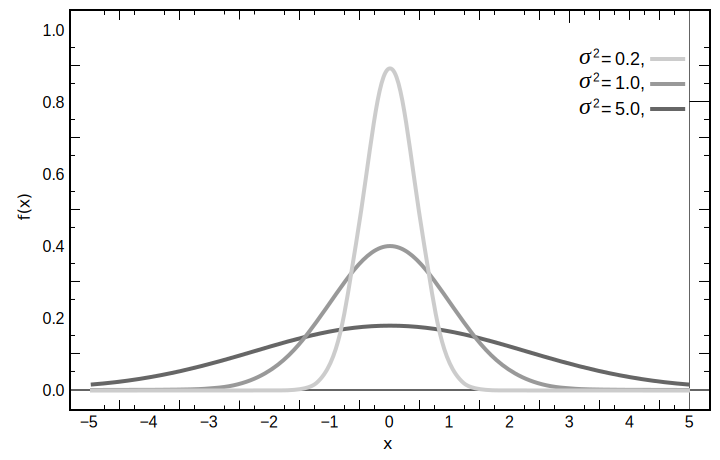
\includegraphics[width=\textwidth]{figs/Normal_Distribution_PDF}
	\caption{Normal distribution for different variances and $\mu=0$.}
	\label{fig:Normal_Distribution_PDF}
\end{figure}

The mean is calculated by
\begin{equation}
\mu=\int_{-\infty}^{\infty}xf(x)dx
\end{equation}
or in other words, each possible value $ x$ is weighted by its likelihood and added up.

The variance is calculated by
\begin{equation}
\sigma^2=\int_{-\infty}^{\infty}(x-\mu)^2f(x)dx
\end{equation}
or in other words, we calculate the deviation of each random variable from the mean, square it, and weigh it by its likelihood. Although it is tantalizing to perform this calculation also for the double dice experiment, the resulting value is questionable, as the double dice experiment does not follow a Normal distribution. We know this, because we actually enumerated all possible outcomes. For other experiments, such as grades in the classes you are taking, we don't know what the real distribution is.


\subsection{Normal distribution in two dimensions}
The Normal Distribution is not limited to random processes with only one random variable. For example, the X/Y position of a robot in the plane is a random process with two dimensions. In case of a multi-variate distribution with $k$ dimensions, the random variable $ X$ is a k-dimensional vector of random variables, $ \mu$ is a k-dimensional vector of means, and $ \sigma$ gets replaced with $ \Sigma$,  a k-by-k dimensional \emph{covariance matrix}\index{Covariance Matrix} (a matrix that carries the variances of each random variable in its diagonal).

\section{Conditional Probabilities and Bayes Rule}\label{sec:bayesrule}
Let $A$ and $B$ be random events with probabilities $P(A)$ and $P(B)$. We can now say that the probability $P(A \cap B)$ that event $A$ \emph{and} $B$ happen is given by
\begin{equation}\label{eq:conditionalprob}
P(A \cap B)=P(A)P(B|A)=P(B)P(A|B)
\end{equation}
Here, $P(B|A)$ is the \emph{conditional probability}\index{Conditional Probability} that $B$ happens, knowing that event $A$ happens. Likewise, $P(A|B)$ is the probability that event $A$ happens given that $B$ happens.

Bayes' Rule\index{Bayes' Rule} relates a conditional probability to its inverse. In other words, if we know the probability of event $A$ to happen given that event $B$ is happening, we can calculate the probability of $B$ to occur given that $A$ is happening. Bayes' rule can be derived from the simple observation that the probability of $A$ and $B$ to happen together ($P(A \cap B)$) is given by $P(A)P(B|A)$ or the probability of $A$ to happen and the probability of $B$ to happen given that $A$ happens (Equation \ref{eq:conditionalprob}). 
From this, deriving Bayes' rule is straightforward:
\begin{equation}
P(A|B)=\frac{P(A)P(B|A)}{P(B)}
\end{equation}
In words, if we know the probability that $B$ happens given that $A$ happens, we can calculate that $A$ happens given that $B$ happens. 

\section{Sum of two random processes}\label{sec:convolution}
Let $X$ and $Y$ be the random variables associated with the numbers shown on two dice (see above), and $Z=X+Y$. With $P(X=x)$, $P(Y=y)$, and $P(Z=z)$ being the probabilities associated with the random variables taking specific values $x,y$ or $z$. Given $z=x+y$, the event $Z=z$ is the union of the independent events $X=k$ and $Y=z-k$. We can therefore write
\begin{equation}
P(Z=z)=\sum_{k=-\infty}^{\infty}P(X=k)P(Y=z-k)
\end{equation}
which is the exact definition of a \emph{convolution}\index{Convolution}, also written as 
\begin{equation}
P(Z)=P(X)\star P(Y)
\end{equation}

Numerically calculating the convolution always works, and can be done analytically for some probability distributions. 

Conveniently, the convolution of two Gaussian distributions is again a Gaussian distribution with a variance that corresponds to the sum of the variances of the indivdiual Gaussians. 

\section{Linear Combinations of Independent Gaussian Random Variables}\label{sec:lcombrandom}
Let $X_1$, $X_2$, $\ldots$, $X_n$ be $n$ independent random variables with means $\mu_1$, $\mu_2$, $\ldots$, $\mu_n$ and variances $\sigma_1^2$, $\sigma_2^2$, $\ldots$, and $\sigma^2_n$. Let $Y$ be a random variable that is a linear combination of $X_i$ with weights $a_i$ so that $Y=\sum_{i=1}^na_iX_i$. 

As the sum of two Gaussian random variables is again a Gaussian, $Y$ is Gaussian distributed with a mean \begin{equation}
\mu_Y=\sum_{i=1}^na_i\mu_i
\end{equation}
and a variance
\begin{equation}
\sigma_Y^2=\sum_{i=1}^na_i^2\sigma_i^2
\end{equation}  



\section{Testing Statistical Significance}\label{sec:stattest}
Robotics is an experimental discipline. This means that algorithms and systems you develop need to be validated by real hardware experiments. Doing an experiment to validate your hypothesis is at the core of the scientific method and doing it right is a discipline on its own. The key is to show that your results is not simply a result of chance. In practice, this is impossible to show. Instead, it is possible to express the likelihood that your results have not been obtained by chance. This is known as the statistical significance level. How to calculate the statistical significance level depends on the problem you are studying. This section will introduce three common problems in robotics:

\begin{enumerate}
\item testing whether data is indeed distributed according to a specific distribution
\item testing whether two sets of data are generated from different distributions
\item testing whether true-false experiments are a sequence of luck or not
\end{enumerate}

\subsection{Null Hypothesis on Distributions}
The Null Hypothesis is a term from the statistical significance literature and formally captures your main claim. A statistical test can either reject the Null Hypothesis or fail to reject it. It can never be proven as there will always be a non-zero probability that all your experiments are just a lucky coincidence. The statistical significance level of a Null Hypothesis is known as the p-value.

An import class of Null Hypothesis are on the distribution of data. Consider the following example from Lab 1 (message passing in ROS). Students were asked to experimentally study the time it takes to pass a message from one process to another:

\begin{framed}
Histogram of the time it takes to send a ROS message from one process to another based on 10 trials.
\end{framed}

We observe three peaks in this Histogram. What can we say about message passing times? For example
\begin{itemize}
\item H0: Message passing times follow a Gaussian distribution.
\item H0: Message passing times follow a bi-modal distribution.
\item H0: Message passing times follow a log-normal distribution.
\end{itemize}

The first Null Hypothesis implies that messages take sometimes a little longer and sometimes a little shorter, but have an average and a variance. The second Null Hypothesis implies that usually messages take some low average time, but occasionally are delayed due to the influence of some other process, for example operating system duties. You can now test each of these hypotheses by calculating the parameters of the distribution to expect and calculate the joint probability that each of your measurements are actually drawn from this distribution. You will find, that all of the above hypotheses are almost equally likely. Together, none of your tests will reject your hypothesis. You therefore will need more data:

\begin{framed}
Histogram of message passing times in ROS based on a 1000 trials.
\end{framed}

You can now again calculate parameters for each distribution you suspect. For example, you can calculate the mean and variance of this data and plot the resulting Gaussian distribution. In this example, the Gaussian distribution will have a mean slightly offset to the right of the peak. You can also fit the data to a log-normal distribution. You can now calculate the likelihood for the data actually be drawn from either of the two distributions. You will see that the joint probability (the product of all likelihoods) for all data points is actually much higher than that for any Gaussian distribution or any bimodal distribution that you are able to fit.

Formally, this can be done by following Pearsons $ \chi^2$-Test (read Chi-Squared Test). This test calculates a value that will approximate a $ \chi^2$-distribution from all samples and the likelihood of that sample based on the expected distribution. Plugging the resulting value into the $ \chi^2$-distribution leads to the statistical significance level (or p-value).

The value of the test-statistic is calculated as follows:
\begin{equation}
\chi^2 = \sum_{i=1}^{n} \frac{(O_i - E_i)^2}{E_i}
\end{equation}
where
\begin{itemize}
\item $ \chi^2$ = Pearson's cumulative test statistic, which asymptotically approaches a chi-squared distribution.
\item $ O_i$ = an observed frequency in the data histogram
\item $ E_i$ = an expected (theoretical) frequency, asserted by the null hypothesis, i.e., the distribution you think the data should follow
\item n = the number of samples.
\end{itemize}
This example also illustrates how statistical tests can be used to determine if you have enough data. If you don't, you will get very poor p-values.  In practice, it is up to you what likelihood you determine to be significant. Standard significance levels are 10\%, 5\% and 1\%. If you are unsatisfied with your p-values you can collect more data and check, whether your p-value improves.

\subsection{Testing whether two distributions are independent}
Testing whether the data of two experiments are independent is probably the most common statistical test. For example, you might run 10 experiments using algorithm 1 and 10 experiments using algorithm 2. It is up to you to show that the resulting distributions are indeed statistically significantly different. In other words, you need to show that the differences between the algorithm indeed lead to a systematic improvement, and that it was not purely luck that one set of experiments turned out ``better'' than another.

If you have good reasons to believe that your data is normal distributed, there exist a series of simple tests. For example, to test whether two sets of data are distributed with Gaussian distributions that have the same mean, can be done using Student's t-test. A generalization of Student's t-test to 3 or more groups is ANOVA. These tests have to be done with care as most distributions in robotics are not normal distributed. Examples where  Gaussian distributions are commonly assumed are sensor noise on distance measurements such as obtained by infrared or odometry.

If data is not Gaussian distributed, there exist a series of numerical tests to test the likelihood that two distributions are independent. For example, you could test the message passing time with and without running some computationally expensive image processing routines. You can then test whether the additional computation affects message passing time. If it does, both distributions need to be significantly different. Just using Student's t-test does not work as the distributions are not Gaussian!

Instead, testing whether two sets of data have the same mean, needs to be done numerically. A common test is Mann-Wilcoxon's Ranked Sum test. An implementation of this test is part of most mathematical calculation programs such as Matlab or Mathematica. An algorithm to calculate this test statistic and the corresponding p-values is available on the Wikipedia page above. An extension of the Mann-Wilcoxon's Ranked Sum test for 3 or more groups is the Kruskal-Wallis one-way analysis of variance test.

\subsection{Statistical Significance of True-False Tests}
There exists a class of experiments that do not lead to distributions, but result in simple true-false outcomes. For example, a question one might ask is ``does the robot correctly understand a spoken command''. This class of experiments is captured by the Lady tasting tea example. Here, a lady claims that she can identify the brewing method of a cup of tea: tea prepared by first adding milk and tea prepared by later adding milk. Unfortunately, it is easy to cheat as the likelihood of guessing right is 50\%. Testing the hypothesis that the lady can indeed differentiate the two brewing methods therefore requires to conduct a series of experiments to reduce the likelihood of winning by guesswork. In order to do this, one needs to calculate the number of total permutations (or, possible outcomes over the entire series of experiments). For example, one could present the lady 8 cups of tea, 4 brewed one way and four the other. One can now enumerate all possible outcomes of this experiment, ranging from all cups guessed correctly to all cups guessed wrong. There are a total of 70 possible outcomes (see the example provided here). Guessing all cups correctly has now a likelihood of 1/70 or 1.4\%. The likelihood to make a single mistake (16 possible outcomes in this example) is around 23\%.

\subsection{Summary}
Statistical significance test allow you to express the likelihood that your experiment is just the result of chance. There exist different tests for different underlying distributions. Therefore, your first task is to convincingly argue what the underlying distribution of your data is. Formally testing how your data is distributed can be achieved using the Chi-Square Test. In order to test whether two sets of data are coming from two different distributions can then be achieved using Student's t-test (if the distribution is Gaussian) or using the Mann-Wilcoxon Ranked Sum test if the probability distribution is non-parametric.
